\documentclass[11pt]{standalone}
\usepackage{amssymb}
\usepackage{amsmath}
\usepackage[no-math]{fontspec}
\usepackage{unicode-math}
\usepackage{libertinus}
\usepackage{pgf,xcolor}
\usepackage{tikz}
\usetikzlibrary{arrows.meta, backgrounds}
\usepackage{pgfplots}
\pgfplotsset{compat=newest}

\definecolor{my_darkgray}{HTML}{484949}
\definecolor{my_lightgray}{HTML}{F3F4F4}
\definecolor{my_darkblue}{HTML}{005A94}
\definecolor{my_lightblue}{HTML}{CCDEE9}
\definecolor{my_yellow}{HTML}{FFEC7F}
\definecolor{my_red}{HTML}{E60000}
\definecolor{my_orange}{HTML}{E87846}

\begin{document}
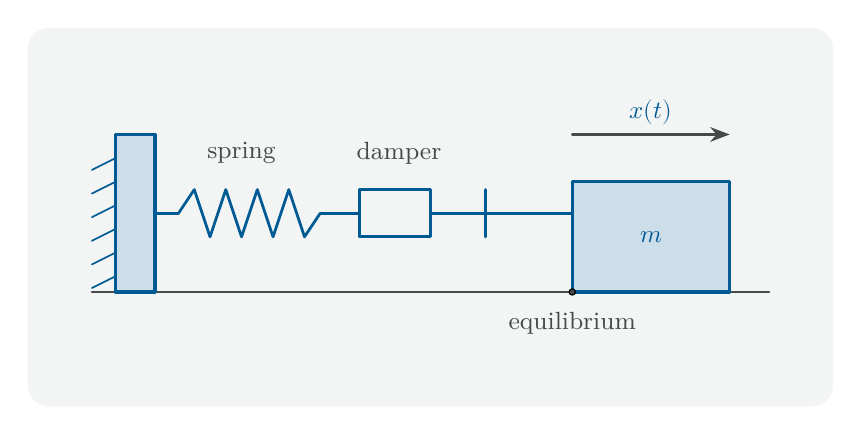
\begin{tikzpicture}[
    show background rectangle,
    background rectangle/.style={fill=my_lightgray, rounded corners=8pt},
    inner frame sep=0.8cm,
    line cap=round,
    line join=round,
    >=Stealth,
    every node/.style={font=\small}
]

% Global scale
\begin{scope}[x=1cm,y=1cm]

% Ground line
\draw[line width=0.9pt, draw=my_darkgray]
    (-0.3,0) -- (8.3,0);

% Fixed wall on the left
\fill[my_lightblue]
    (0,0) rectangle (0.5,2.0);
\draw[line width=1.2pt, draw=my_darkblue]
    (0,0) rectangle (0.5,2.0);

% Hatch the wall to indicate fixed support
\foreach \y in {0.2,0.5,...,1.8} {
  \draw[draw=my_darkblue, line width=0.6pt]
    (0,\y) -- (-0.3,\y-0.15);
}

% Mass block on the right
\fill[my_lightblue]
    (5.8,0) rectangle (7.8,1.4);
\draw[line width=1.2pt, draw=my_darkblue]
    (5.8,0) rectangle (7.8,1.4);

% Mass label
\node[my_darkblue] at (6.8,0.7) {$m$};

% Spring between wall and damper
% Anchor points: from x = 0.5 to x = 2.7 at height 1.0
\coordinate (spring-left)  at (0.5,1.0);
\coordinate (spring-right) at (2.7,1.0);

% Short straight segment at left end
\draw[line width=1.0pt, draw=my_darkblue]
    (spring-left) -- ++(0.3,0);

% Manually drawn zigzag spring
\draw[line width=1.0pt, draw=my_darkblue]
    (0.8,1.0) --
    (1.0,1.3) --
    (1.2,0.7) --
    (1.4,1.3) --
    (1.6,0.7) --
    (1.8,1.3) --
    (2.0,0.7) --
    (2.2,1.3) --
    (2.4,0.7) --
    (2.6,1.0);

\draw[line width=1.0pt, draw=my_darkblue]
    (2.6,1.0) -- (spring-right);

% Spring label
\node[my_darkgray, above] at (1.6,1.5) {spring};

% Damper between spring and mass
% Anchor points: from x = 2.7 to x = 5.8 at height 1.0
\coordinate (damper-left)  at (2.7,1.0);
\coordinate (damper-right) at (5.8,1.0);

% Left fixed plate of damper
\draw[line width=1.0pt, draw=my_darkblue]
    (damper-left) -- ++(0.4,0);
\draw[line width=1.0pt, draw=my_darkblue]
    (3.1,1.3) -- (3.1,0.7);

% Damper body
\draw[line width=1.0pt, draw=my_darkblue]
    (3.1,1.3) -- (4.0,1.3) --
    (4.0,0.7) -- (3.1,0.7) -- cycle;

% Piston rod and right plate
\draw[line width=1.0pt, draw=my_darkblue]
    (4.0,1.0) -- (4.7,1.0);
\draw[line width=1.0pt, draw=my_darkblue]
    (4.7,1.3) -- (4.7,0.7);
\draw[line width=1.0pt, draw=my_darkblue]
    (4.7,1.0) -- (damper-right);

% Damper label
\node[my_darkgray, above] at (3.6,1.5) {damper};

% Displacement axis and label x(t)
\draw[->, line width=0.9pt, draw=my_darkgray]
    (5.8,2.0) -- (7.8,2.0);
\node[my_darkblue, above] at (6.8,2.0) {$x(t)$};

% Origin marker (equilibrium position) on ground line, label above
\draw[fill=my_darkgray] (5.8,0) circle (0.04);
\node[my_darkgray] at (5.8,-0.4) {equilibrium};

% Positive direction arrow near ground, left side
%\draw[->, line width=0.8pt, draw=my_darkgray]
%    (1.0,-0.4) -- (2.0,-0.4);
%\node[my_darkgray, above] at (1.6,-1.0) {positive $x$};

\end{scope}
\end{tikzpicture}
\end{document}